\begin{frame}{Autour du monde}
  \only<1>{
    En groupes de 4, chosissez l'un des pays ou régions au-dessous, allez à \href{https://www.ledevoir.com}{Le Devoir} (\href{https://www.ledevoir.com}{www.ledevoir.com}), cherchez un ou plusieurs articles qui décrit une inégalité sociale dans ce pays ou cette région, lisez-le.s et préparez un bref résumé \gloss{short summary} de l'article à présenter à la classe.
  }
  \begin{columns}
    \column{0.4\textwidth}
      \begin{enumerate}
        \item Haïti
        \item Sénégal
        \item Québec
        \item Vietnam
        \item Algérie
        \item France
      \end{enumerate}
    \column{0.6\textwidth}
      \begin{center}
        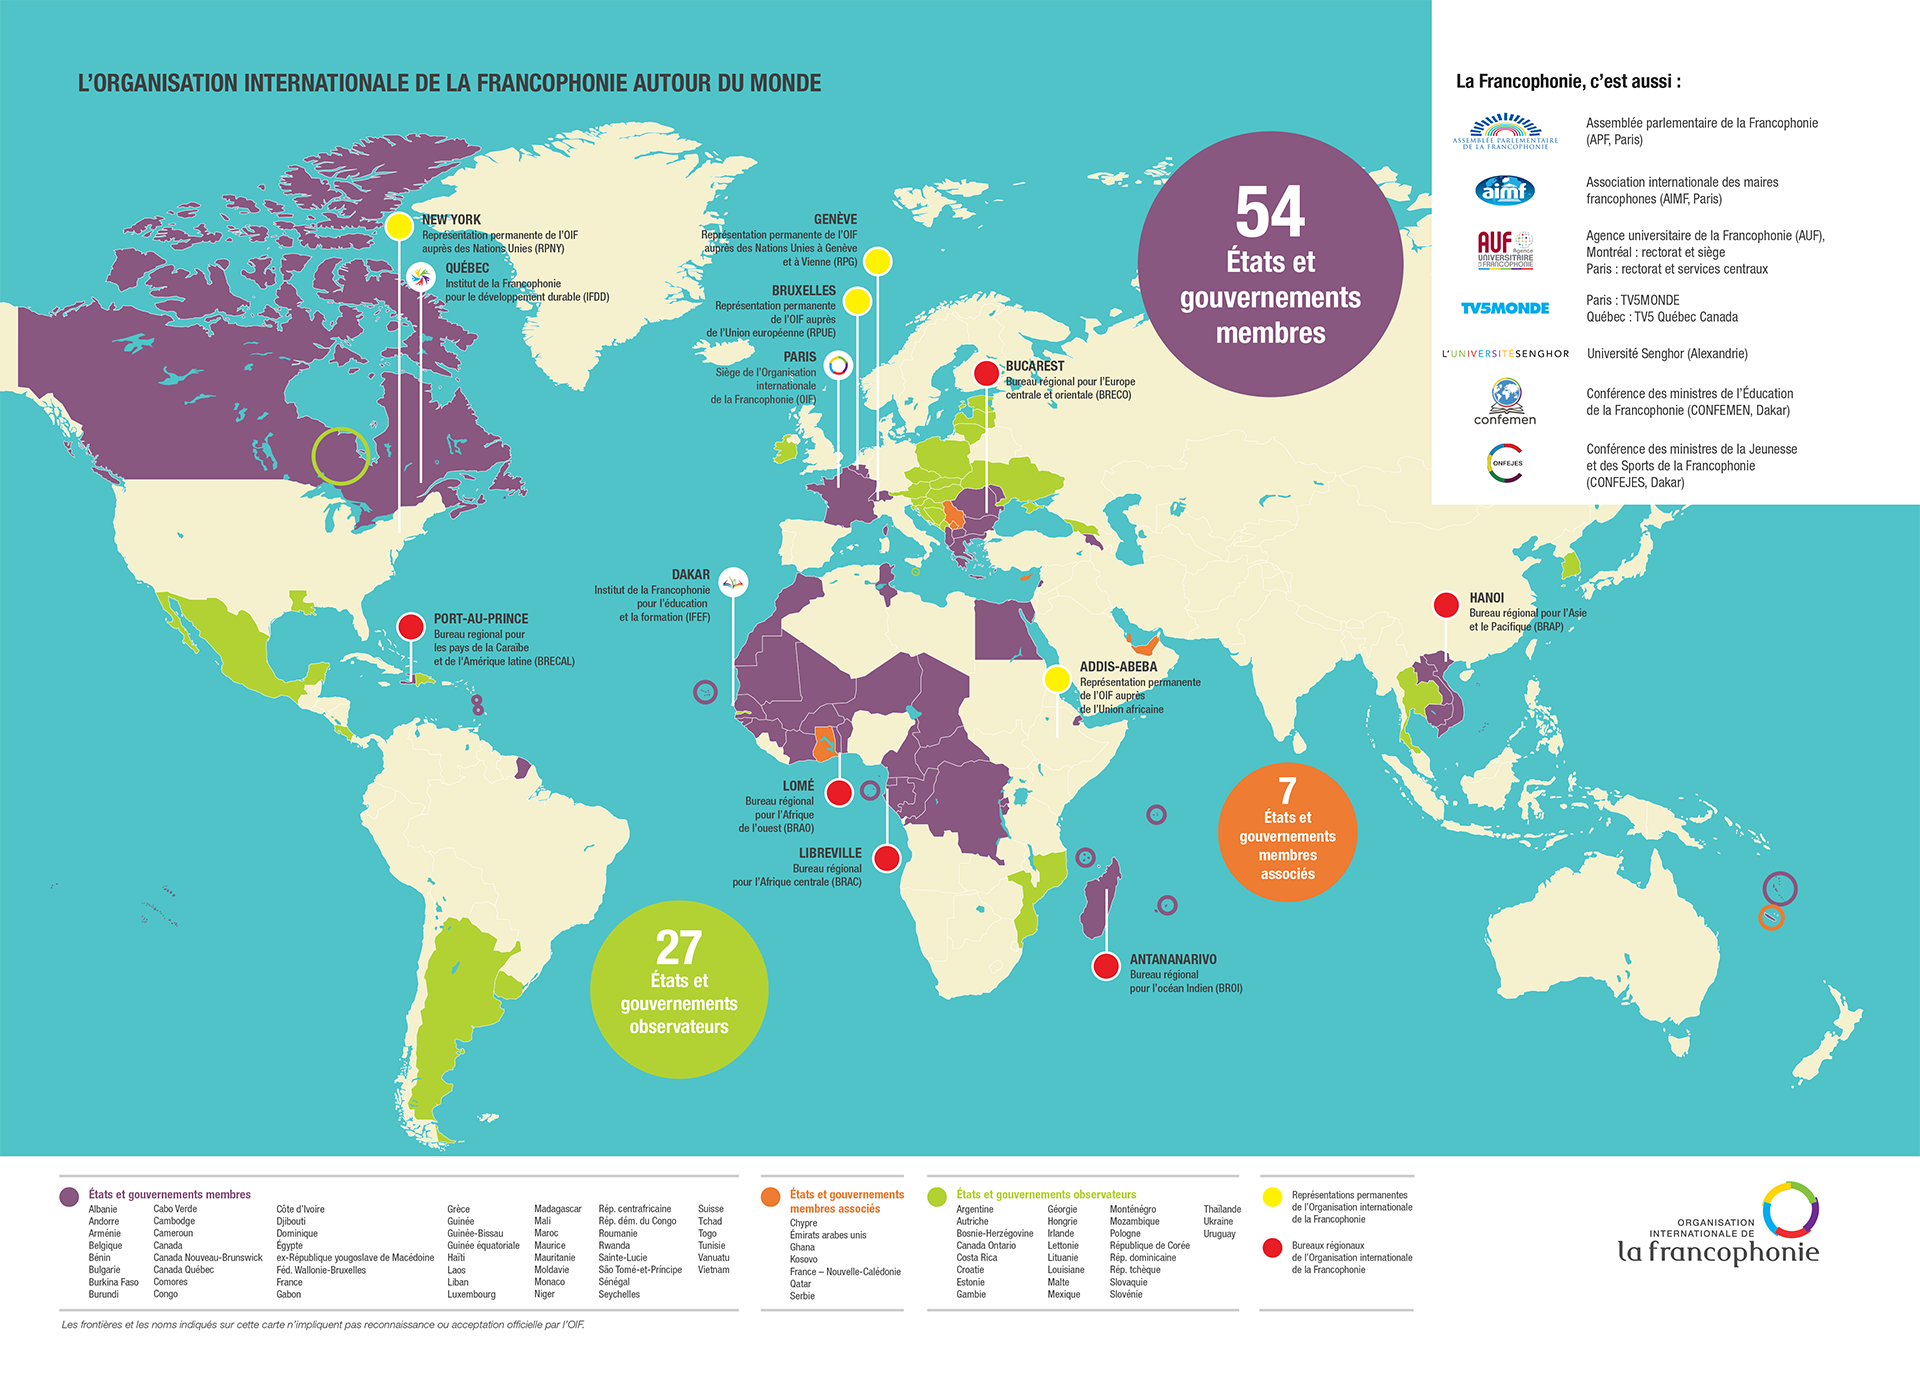
\includegraphics[scale=0.1]{francophonie.png}
      \end{center}
  \end{columns}
  \only<2>{
    Maintenant, pendant que vous écoutez les résumés, écrivez une question à poser au groupe.
  }
\end{frame}